\documentclass[10pt]{article}
\usepackage{icmlko}

\icmlmeta{IP 파운데이션 월드모델}{107}{가를 값은 있는데 가를 수가 없다}{두 지표의 상관이 $-$0.245라 제품용 설정을 따로 둘 값이 있어 보였는데, 고르는 순간 아무것도 안 고르는 현행에 진다}

\begin{document}

\twocolumn[
\icmlheader

\begin{abstract}
노트 106이 처음으로 \textbf{판정치와 팝업이 반대로 가는} 지렛대를 냈다
(시간 분할에서 $+$0.0188 대 $-$0.0301). 그러면 설정을 갈라야 하나 --- 연구용은
판정치를, 제품용은 팝업을 최대로. \textbf{가르기 전에 가를 값이 있는지부터
쟀다.} 설정 스무 개에서 두 지표를 다 냈다. \textbf{거의 무관하다}
($r{=}-$0.245). 순위도 뒤섞인다 --- 판정치 최고는 ``설명문 고유 $k{=}3$''
($+$0.4165)인데 그 설정의 팝업은 $+$0.4578로 여섯째이고, 팝업 최고는
``$k{=}1$ 전역''($+$0.4736)인데 그 설정의 판정치는 $+$0.3891로 \emph{꼴찌에서
둘째}다. 전체 자료에서 팝업 기준으로 고르면 $+$0.0157을 번다.
\textbf{그런데 고를 수가 없다.} 반쪽 분할 일곱에서 A반 팝업으로 고르고 B반
팝업으로 재면 판정치로 고른 것보다 \textbf{$-$0.0213} 나쁘고 이긴 분할이
3/7이다. 한 분할에서는 $-$0.1395까지 진다. 그리고 \textbf{둘 다 아무것도 안
고르는 현행에 진다} --- 현행 $+$0.5091, 판정치로 고른 것 $+$0.5031, 팝업으로
고른 것 $+$0.4818. 이유는 노트 92가 이미 셌다 --- \textbf{팝업 75건은 도구를
\emph{쓰기}엔 충분하지만 설계를 \emph{판정}하기엔 부족하다}(510건 필요).
설정을 가르는 것 자체가 팝업으로 내리는 설계 결정이므로 같은 벽에 걸린다.
\textbf{설정은 하나로 간다.} 이 프로젝트에서 ``고르면 진다''의 일곱째
사례이고, 처음으로 \emph{제품 결정}에서 그렇다.
\end{abstract}
]

\begin{figure*}[t]
\centering
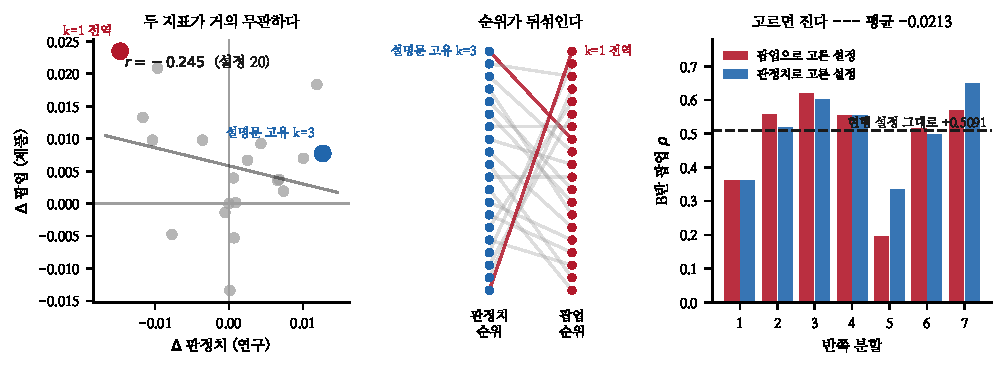
\includegraphics[width=\textwidth]{figs/sp.pdf}
\caption{왼쪽 --- 두 지표가 거의 무관하다. 가운데 --- 순위가 뒤섞인다.
오른쪽 --- 고르면 진다.}
\end{figure*}

\section{가를 값은 있어 보인다}

설정 스무 개를 만들었다 --- 성분 수 셋, 설명문 축 넷, 표지 축 둘, 문장 수,
입장료 공통 셋, 사상 셋, 조합 둘, 그리고 현행.

\begin{table}[t]
\centering\tsize
\caption{두 지표. 위쪽은 판정치 상위, 아래쪽은 팝업 상위.}
\begin{tabular}{lrr}
\toprule
& $\Delta$판정치 & $\Delta$팝업 \\
\midrule
\textbf{설명문 고유 $k{=}3$} & \textbf{$+$0.0127} & $+$0.0077 \\
설명문 출처6 $k{=}3$ & $+$0.0119 & $+$0.0183 \\
입장료 공통 & $+$0.0100 & $+$0.0070 \\
설명문 $c_1$ 고유 & $+$0.0074 & $+$0.0019 \\
\midrule
\textbf{$k{=}1$ 전역} & \textbf{$-$0.0147} & \textbf{$+$0.0235} \\
입장료 공통 $k{=}3$ & $-$0.0096 & $+$0.0209 \\
표지 밝기 고유 & $-$0.0116 & $+$0.0133 \\
표지 고유 $k{=}2$ & $-$0.0103 & $+$0.0098 \\
\midrule
\multicolumn{2}{l}{두 지표의 상관} & \textbf{$r{=}-$0.245} \\
\bottomrule
\end{tabular}
\end{table}

\claimx{두 지표가 \textbf{거의 무관하다}($r{=}-$0.245). 판정치 최고 설정의
팝업은 스무 개 중 여섯째이고, 팝업 최고 설정($k{=}1$ 전역)의 판정치는
꼴찌에서 둘째다. \textbf{전체 자료에서 팝업 기준으로 고르면 $+$0.0157을
번다.}}{스무 개는 내가 고른 목록이다. 다른 설정군이면 상관이 달라질 수 있다.}

\section{그런데 고를 수가 없다}

$+$0.0157은 \emph{평가한 자료에서 고른} 값이다. 노트 92 · 101 · 102가 같은
함정을 세 번 보였으므로 반쪽 검정을 건다 --- \textbf{A반에서 고르고 B반에서
잰다.}

\begin{table}[t]
\centering\tsize
\caption{반쪽 분할 일곱. B반 팝업 $\rho$.}
\begin{tabular}{lrrr}
\toprule
& 팝업으로 고름 & 판정치로 고름 & 차 \\
\midrule
1 & $+$0.3625 & $+$0.3625 & $+$0.0000 \\
2 & $+$0.5573 & $+$0.5199 & $+$0.0374 \\
3 & $+$0.6203 & $+$0.6008 & $+$0.0195 \\
4 & $+$0.5539 & $+$0.5539 & $+$0.0000 \\
\textbf{5} & $+$0.1961 & $+$0.3356 & \textbf{$-$0.1395} \\
6 & $+$0.5147 & $+$0.4987 & $+$0.0160 \\
\textbf{7} & $+$0.5677 & $+$0.6504 & \textbf{$-$0.0827} \\
\midrule
평균 & \textbf{$+$0.4818} & $+$0.5031 & \textbf{$-$0.0213} \\
\midrule
\multicolumn{2}{l}{\textbf{현행 설정 그대로}} & \textbf{$+$0.5091} & \\
\bottomrule
\end{tabular}
\end{table}

\claimx{\textbf{제품용 설정을 따로 고르면 진다.} 팝업으로 고른 것이 판정치로
고른 것보다 $-$0.0213 나쁘고, \textbf{둘 다 아무것도 안 고르는 현행에 진다}
($+$0.5091). 한 분할에서는 $-$0.1395까지 벌어진다.}{일곱 분할이고 둘은
$\pm$0.0000이다(같은 설정을 골랐다). 실제로 갈린 분할은 다섯이고 그중 셋이
양수다 --- \textbf{평균을 만드는 것은 두 개의 큰 음수}이므로 ``항상 진다''가
아니라 ``크게 질 때가 있다''가 맞다.}

\begin{quote}\fontsize{9.5}{11.5}\selectfont
\textbf{이유는 이미 세어 놓았다.} 노트 92가 팝업 표본이 무엇을 사고 무엇을
못 사는지 갈랐다 --- 도구를 \emph{쓰는} 데는 50건, 설계를 \emph{판정}하는
데는 510건. 지금 75건이다. \textbf{설정을 가르는 것 자체가 팝업으로 내리는
설계 결정}이므로 같은 벽에 걸린다. 반쪽 분할에서는 37건이니 더 심하다.
\end{quote}

\section{그래서 하나로 간다}

\begin{table}[t]
\centering\tsize
\caption{결정.}
\begin{tabular}{ll}
\toprule
연구용 설정 & 두지 않는다 \\
제품용 설정 & 두지 않는다 \\
\textbf{현행 하나} & \textbf{유지} \\
\bottomrule
\end{tabular}
\end{table}

\claimx{노트 106이 연 물음이 닫힌다 --- \textbf{판정치와 팝업이 갈려도 설정을
가르지 않는다.} 가를 값은 있지만($r{=}-$0.245) 그 값을 집을 표본이 없다.}
{팝업 레코드가 510건이 되면 다시 물어야 한다. 그때는 가르는 것이 옳을 수
있다.}

\begin{quote}\fontsize{9.5}{11.5}\selectfont
이 프로젝트에서 ``고르면 진다''의 일곱째 사례다 --- 노트 67(작은 표본 배선) ·
80(잡음 부분집합) · 82(도메인 제거) · 92(성분 수) · 98(슬롯 완전성) ·
101(성분 규칙) · 102(라벨 상관 선별), 그리고 여기. \textbf{처음으로 제품
결정에서 그렇다.} 앞의 일곱은 전부 모형 내부의 선택이었고, 이번 것은 ``도구를
어떤 설정으로 돌릴 것인가''다.
\end{quote}

\section{한계}

\begin{itemize}[leftmargin=1.1em,itemsep=0.15em]
\item 설정 스무 개가 내가 고른 목록이다. 더 넓히면 갈릴 값이 커질 수 있다.
\item 반쪽 분할이 일곱이고 그중 둘은 두 기준이 같은 설정을 골랐다. 실제
      대비는 다섯 분할이다.
\item $-$0.0213이 두 개의 큰 음수에서 온다. 일곱 분할의 중앙값은 $+$0.0000이고
      실제로 갈린 다섯만 보면 중앙값이 $+$0.0160이다 --- \textbf{``고르면
      평균적으로 진다''이지 ``항상 진다''가 아니다.}
\item 반쪽 분할이 팝업을 37건으로 줄인다. 노트 106이 지적한 문제가 여기서도
      그대로다 --- 시간 분할로 다시 하면 다를 수 있다.
\item 노트 105 · 106이 남긴 접근 허용 폭과 미디어 홍보 수집은 세 노트째 미룸.
\end{itemize}

\section{다음}

\begin{enumerate}[leftmargin=1.3em,itemsep=0.15em]
\item \textbf{같은 물음을 시간 분할로} --- 반쪽 분할은 팝업을 37건으로 줄인다.
      시간 분할은 안 줄이므로 결론이 뒤집힐 수 있다. 이 노트의 가장 큰 구멍이다.
\item \textbf{미디어 홍보 덮개율을 채운다}(세 노트째 미룸) --- 다섯 도메인
      0\%인데 잔차 0.727로 나쁘지 않았다. 예고편 유무 · 공식 계정 · 보도
      신호를 긁는다. 축을 \emph{고르는} 것이 아니라 \emph{채우는} 것이므로
      이 노트의 결론과 어긋나지 않는다.
\item \textbf{접근 허용 폭}(노트 105) --- 만화 · 세계애니의 연령 등급이 타깃
      폭과 $+$0.27밖에 안 겹치는 73\%의 정체.
\item 팝업 레코드. 510건이 모든 것을 푼다(노트 92 · 106 · 107).
\end{enumerate}

\vspace{0.6em}
\hrule height 0.3pt
\vspace{0.5em}
{\footnotesize
\textbf{참고문헌}\\[0.3em]
Cawley, G. C., Talbot, N. L. C. (2010). On over-fitting in model selection and
subsequent selection bias in performance evaluation. \emph{JMLR}, 11, 2079--2107.\\[0.15em]
Varoquaux, G. (2018). Cross-validation failure: small sample sizes lead to large
error bars. \emph{NeuroImage}, 180, 68--77.\\[0.15em]
Simpson, E. H. (1951). The interpretation of interaction in contingency tables.
\emph{JRSS B}, 13(2), 238--241.\\[0.15em]
Ben-David, S. et al. (2010). A theory of learning from different domains.
\emph{Machine Learning}, 79(1--2), 151--175.\\[0.15em]
Efron, B., Tibshirani, R. J. (1993). \emph{An Introduction to the Bootstrap}.
Chapman \& Hall.
}

\end{document}
